\usetikzlibrary {arrows}
\usetikzlibrary {shapes.geometric}
\usetikzlibrary {patterns}

\chapter{Background}
First, background of this project is discussed and suitable explanations provide context for the entire project. The broad scope of the project is presented before going into project-specific details in the \textit{Context} chapter.

\section{The Semantic Web}
\hspace*{0.5cm} The Semantic Web is an extension of the World Wide Web (WWW) that allows information on it to be machine-readable \cite{semanticweb}. The concept was founded by Tim Berners-Lee (founder of the WWW) with the idea that machines can easily interpret information available on the WWW. Tim Berners-Lee initially thought of this idea in 1999 stating ``I have a dream for the Web [in which computers] become capable of analysing all the data on the Web – the content, links, and transactions between people and computers. A `Semantic Web'" \cite{berners-TBLBook}. Ultimately, the semantic web aims to empower the knowledge embedded online so that it can be parsed by machines \cite{semanticweb}. 

An example of these developments can be seen in a data storage project that contains structures interpretable by both humans and machines- Wikidata. Wikidata is a large open knowledge base that is part of the Wikimedia family (including Wikipedia) and is connected to other datasets as well \cite{wikidata}. Data is stored in WikiData using various web data storage methods such as JSON, XML and RDF (Resource Description Framework). The latter is described in more detail in the next section.  

Another example within the project scope is MusicBrainz. MusicBrainz also provides information that is stored using RDF \cite{musicbrainz}. In this case, MusicBrainz's focus is around music so it may be more relevant and provide more specific data for the project. 

\subsection{Resource Description Framework}
\hspace*{0.5cm} Resource Description Framework (RDF) is a method in which data can be stored, similar to how data can be stored in JSON or XML formats. However, the structure of RDF is very different. The general idea of RDF revolves around the concept of linked and connected data so RDF stores data in triples with relationships between data. Data stored in this format is both machine and human-readable, making the reuse and extension of data semantics possible \cite{rdf}. Each triple follows this structure: 

\vspace{-0.1cm}
\begin{center}
\begin{displayquote}
   \textit{subject predicate object}
\end{displayquote} 
\end{center}
\vspace{-0.2cm}

\textbf{Subject:} \\
The subject is the entity that the triple is about or refers to, which is typically a resource. A resource can be a Uniform Resource Identifier (URI- a string that identifies a name or resource on the Internet \cite{sikos_2015}), a physical thing or an abstract concept. 

\textbf{Predicate:} \\
The predicate conveys the relationship between subject and object (i.e. how they are related). 

\textbf{Object:} \\
The object is an entity that the triple describes in relation to the subject. This can also be blank. 

In this project, we will look closer at the Turtle (TTL) format for RDF. A TTL file represents RDF triples with a subject, object and relationship. This format is specifically relevant when representing multiple related RDF triples (RDF Graph) and allows them to be readable by both humans and machines \cite{TTL}.

An example of an RDF statement (in TTL) can be seen below:

\vspace{-0.4cm}
\begin{center}
\lstset
{
    breaklines=true,
    breakatwhitespace=true,
    basicstyle=\linespread{1.5}\ttfamily,
}
\begin{lstlisting}
    <http://www.example.com/Alvin> 
    <http://www.example.com/vocab#studiesAt> 
    <http://www.example.com/KCL>
\end{lstlisting}
\end{center} 
\vspace{-0.3cm}

\noindent In this example, 
\vspace{-0.15cm}
\begin{itemize}
    \itemsep0em 
\item \textbf{The subject is:} \\ \textit{``http://www.example.com/Alvin"}
\item \textbf{The predicate is:} \\ \textit{``http://www.example.com/vocab\#studiesAt"}
\item \textbf{The object is:} \\ \textit{``http://www.example.com/KCL"}
\end{itemize}
\vspace{-0.1cm}

This statement indicates that the entity \textit{``http://www.example.com/Alvin"} studies at the entity \textit{``http://www.example.com/KCL"}, according to the vocabulary defined by \\\textit{``http://www.example.com/vocab"}. However, writing all the various URI links separately is tedious and can look confusing for the human reader so using prefixes as shown below can make it more concise:

\vspace{-0.2cm}
\lstset
{
    breaklines=true,
    breakatwhitespace=true,
    basicstyle=\linespread{1.5}\ttfamily,
}
\begin{center}
\begin{lstlisting}
    @prefix ex: <http://www.example.com/>. 
    @prefix exVocab: <http://www.example.com/vocab#>. 

    ex:Alvin exVocab:studiesAt ex:KCL
\end{lstlisting}
\end{center} 
\vspace{-0.2cm}

This example uses two abbreviations of URIs and has named the alias for these URIs to be `ex' and `exVocab' respectively, simplifying the triple. 

An English translation of the RDF triple is written below: 

\vspace{-0.1cm}
\begin{center}
    \textit{``Alvin studies at KCL".}
\end{center}
\vspace{-0.1cm}

As mentioned previously, RDFs can also be visualised in graph format with numerous relationships between subjects and objects, specifying their relationships. In particular, this project's produced knowledge graph will be in RDF format and be represented in a TTL file. RDFs can be used to describe ontologies, which are described in the next section.

\section{Ontology}
\hspace{0.5cm} An ontology is a conceptual framework for modelling domain knowledge \cite{ontology}. Ontologies make use of RDF triples by having two nodes (the subject and predicate) and an edge (the relationship). They act as models in which real data can be input, so these ontologies can be reused in different contexts and shared between users. These generalised models are ideal for knowledge graph generation because data from different contexts can be displayed in the same way using the same ontology. 

The main components of an ontology are similar to the RDF triples in the previous section but have different names. They involve:

\vspace{-0.15cm}
\begin{itemize}
    \itemsep0em 
\item \textbf{Classes}: \\
A collection of objects or things that are related to each other in some way.

\item \textbf{Relationship}: \\
A link between a class and an attribute that describe how they are related. 

\item \textbf{Attributes}:\\ 
A characteristic or property that a class may have, which is described by the relationship between them.

\end{itemize}
\vspace{-0.15cm}

In relation to RDF statements, a connection between two nodes in an ontology will have subject and object nodes with a connecting edge specified by the predicate. \textit{Figure 2.1}, is an example of a graphical visualisation in the context of a football team:

\begin{figure}[H]
\begin{center}
    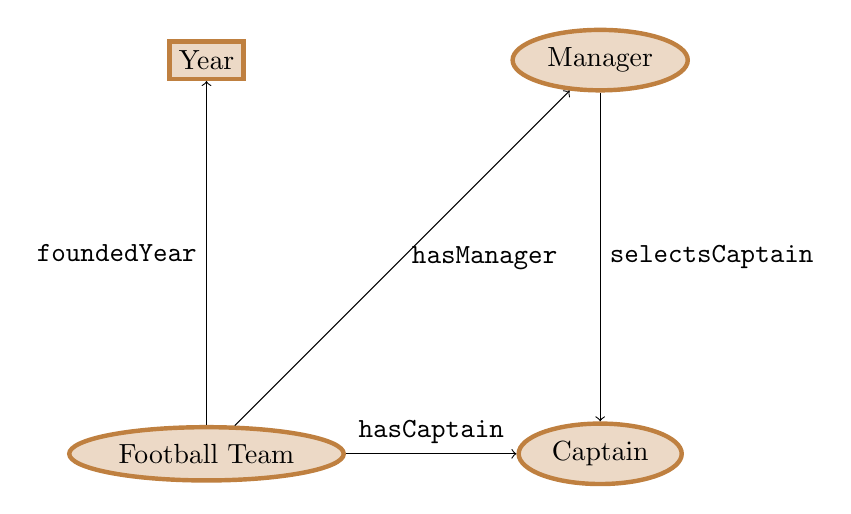
\begin{tikzpicture} [
        circle/.style={draw=brown, ellipse, ultra thick, fill=brown!30},
        square/.style={draw=brown, rectangle, ultra thick, fill=brown!30},
        align=center,
        node distance=5cm ]
    \node[circle] (q1)  {Football Team};
    \node[circle, right of=q1] (q2)  {Captain};
    \draw (q1) edge[->,above] node {\tt hasCaptain} (q2);
    \node[square, above of=q1] (q3) {Year};
    \draw (q1) edge[->,left] node {\tt foundedYear} (q3);
    \node[circle, above of=q2] (q3) {Manager};
    \draw (q1) edge[->,right] node {\tt hasManager} (q3);
    \draw (q3) edge[->,right] node {\tt selectsCaptain} (q2);
    \end{tikzpicture}
\end{center}
\vspace{-0.2cm}
\caption{Example Arsenal Ontology}
\end{figure}
\vspace{-0.15cm}

\textit{Figure 2.1} depicts a Football Team with a Manager and a Captain. The Manager and Captain (of the football team) also have a relationship because the manager selects a specific captain for the football team. The attribute `Year' only describes the `Football Team' class so is denoted as such.

Ontologies are the framework in which knowledge graphs can be constructed and guide the generation of knowledge graphs. 

\subsection{Knowledge Graphs}
\hspace{0.5cm} A knowledge graph is a graph (i.e. data graph) that depicts real-world knowledge or data \cite{knowledgegraph}. Similar to ontologies, knowledge graphs are often represented as a network of interconnected nodes and edges but instead, nodes represent real-world entities (such as people or places) and edges represent the real-world relationships between them (such as `owns' or `discovered'). 

As mentioned, knowledge graphs apply real data from an ontology framework. With a dataset and relevant ontology, we can create specific instances of each ontological relationship. 

Knowledge graphs are used in a variety of real-world applications including search engines, recommendation systems and natural language processors. More detail on these examples are below:

\vspace{-0.1cm}
\begin{itemize}
\itemsep0em 
\item \textbf{Search Engines:} \\Knowledge graphs are used by search engines such as Google to find appropriate results given a search query. Results are interpreted and relevant information is displayed based on relationships between the URIs and meaning of the search term. The most relevant information with regard to the search query is displayed to the user. The method in which a knowledge graph aids a specific search query is called a ``semantic search" and provides more accurate and relevant results. This mirrors how humans tend to think by emulating our natural ability to find associations between data \cite{searchengine}.  

\item \textbf{Recommendation Systems:} \\Knowledge graphs can be used in such systems because there are often many associations between different entities. Recommendation systems use relationships in the knowledge graph to display the most relevant data to the user. 

\item \textbf{Natural Language Processing:}\\ In this context, knowledge graphs are used to establish connections between distinct terms linked within text. A system employing Natural Language Processing may want to understand the meaning of a sentence and be able to interpret and input it into a search query so that relevant results can be found. 
\end{itemize}

An example of a knowledge graph can be in \textit{Figure 2.2}, following the ontology in \textit{Figure 2.1} displayed in the ontology section above:

\begin{figure}[H]
\begin{center}
    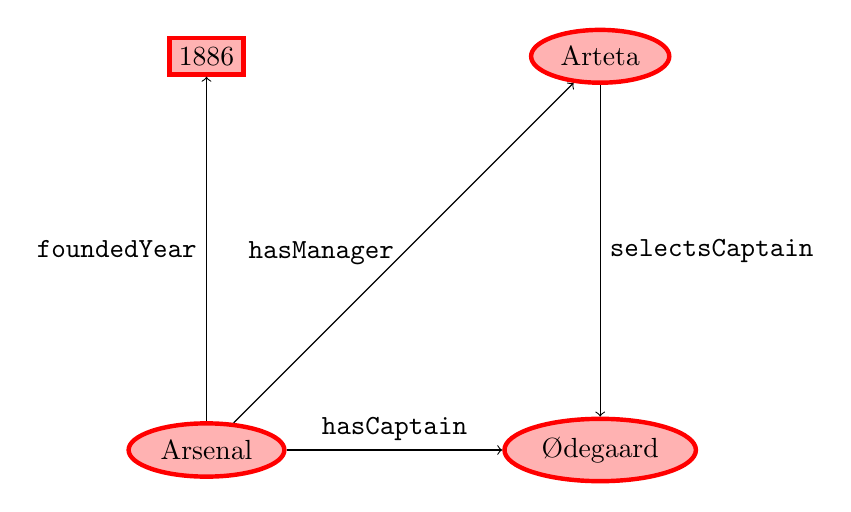
\begin{tikzpicture} [
        circle/.style={draw=red, ellipse, ultra thick, fill=red!30},
        square/.style={draw=red, rectangle, ultra thick, fill=red!30},
        align=center,
        node distance=5cm ]
    \node[circle] (q1)  {Arsenal};
    \node[circle, right of=q1] (q2)  {Ødegaard};
    \draw (q1) edge[->,above] node {\tt hasCaptain} (q2);
    \node[square, above of=q1] (q3) {1886};
    \draw (q1) edge[->,left] node {\tt foundedYear} (q3);
    \node[circle, above of=q2] (q3) {Arteta};
    \draw (q1) edge[->,left] node {\tt hasManager} (q3);
    \draw (q3) edge[->,right] node {\tt selectsCaptain} (q2);
    \end{tikzpicture}
\end{center}
\vspace{-0.4cm}
\caption{Example Arsenal Knowledge Graph}
\end{figure}
\vspace{-0.1cm}

\textit{Figure 2.2} describes Arsenal's men's football team. Arteta is the manager of Arsenal and Arsenal's captain is Ødegaard. Arteta (the manager) also selects the captain. The year Arsenal was founded is displayed in the graph as 1886.

The more linked data we add from the dataset, the larger the knowledge graph will grow.

\section{SPARQL}
\hspace{0.5cm} SPARQL enables us to query RDF data formats and retrieve specific data from large RDF files. SPARQL queries often have the same structure as standard SQL queries. Specific data can be specified and filtered by stating the subject, object and relationship in the query's SELECT and WHERE clause respectively \cite{sparlbook}. An example of a SPARQL Query is shown with an explanation below:

\begin{lstlisting}
PREFIX foaf: <http://xmlns.com/foaf/0.1/>
SELECT ?first_name 
       ?surname
WHERE
  {
    ?person  a          foaf:Person.
    ?person  foaf:name  ?first_name.
    ?person  foaf:surname  ?surname.
  }
\end{lstlisting}
\textit{Example from}: \cite{foaf}

\medskip
Here, the shortcut `foaf' (friend of a friend) is used, which is often used to describe people, their characteristics, relationships and other information about them \cite{foaf}.

The \textbf{SELECT} part of the query extracts all the first and last names of people in the queried TTL file with RDF type \textit{foaf:Person}. The selected people must also have a name and surname specified in the file.

The \textbf{WHERE} clause of the query specifies that the queried variable \textit{?person} belongs to the RDF class \textit{foaf:Person}. The \textit{?person} should also possess both a name and a surname represented by the property \textit{foaf:name} and \textit{foaf:surname} respectively.

In conclusion, if the query were to be executed in an appropriate RDF document, the result would display the first and last names of all individuals in the TTL file of type \textit{foaf:Person}. Moreover, the individuals outputted will have both a name and surname property.
